\setlength{\columnsep}{3pt}
\begin{flushleft}
	
	\begin{itemize}
		\item VG are segmented into small, fixed-size chunks called \textbf{physical extents} (PE).
		\item LV are created by adding up these PEs in VG.
		\begin{figure}[h!]
			\centering
			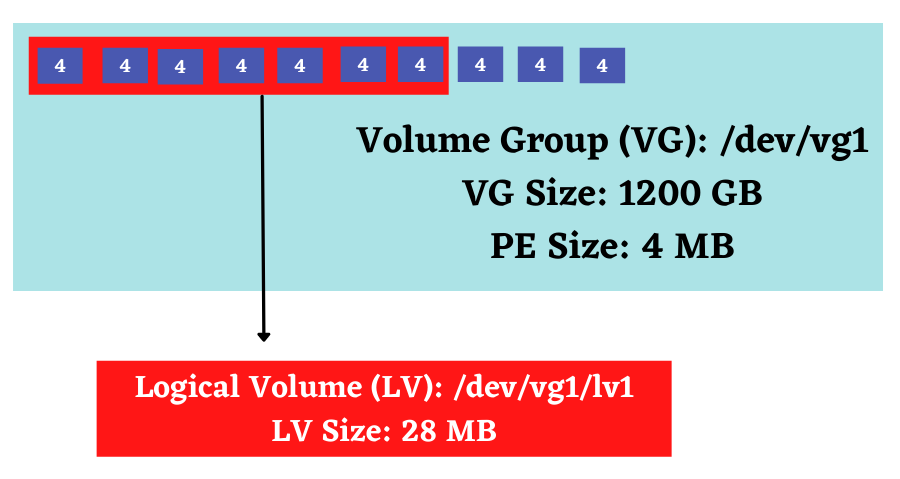
\includegraphics[scale=.55]{content/chapter9/images/pe.png}
			\caption{Physical extend}
			\label{fig:pe_le}
		\end{figure}	
		\item \textbf{Default PE size is 4MB}.
		\item Command to check PE size of VG:
		\begin{figure}[h!]
			\centering
			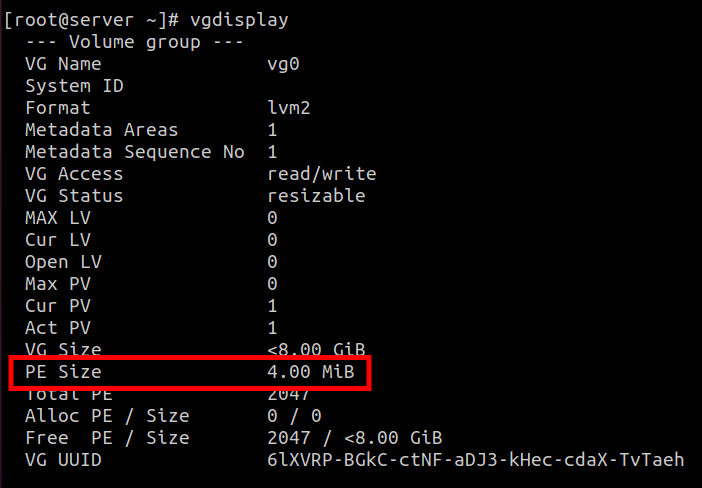
\includegraphics[scale=.4]{content/chapter9/images/p2.png}
			\caption{Sample output of vgdisplay}
			\label{fig:PE size}
		\end{figure}
		\newpage
		\item \textbf{You can change the PE size} for your volume group at the time of VG creation
		\newline
		Command to change PE size:
		\newline
		\textbf{vgcreate -s}: The \textbf{-s} option allows to change the PE size at the time of VG creation
		\bigskip 
		\begin{tcolorbox}[breakable,notitle,boxrule=-0pt,colback=pink,colframe=pink]
			\color{black}
			\fontdimen2\font=0.8em
			Syntax: vgcreate -s PE\_size vg\_name pv\_name
			\fontdimen2\font=4pt
		\end{tcolorbox}
		
		Eg: Resize the filesystem of logical volume:
		\begin{tcolorbox}[breakable,notitle,boxrule=-0pt,colback=black,colframe=black]
			\color{green}
			\fontdimen2\font=1em
			\# vgcreate -s 8 vg0 /dev/sdb
			\fontdimen2\font=4pt
		\end{tcolorbox}
		\begin{figure}[h!]
			\centering
			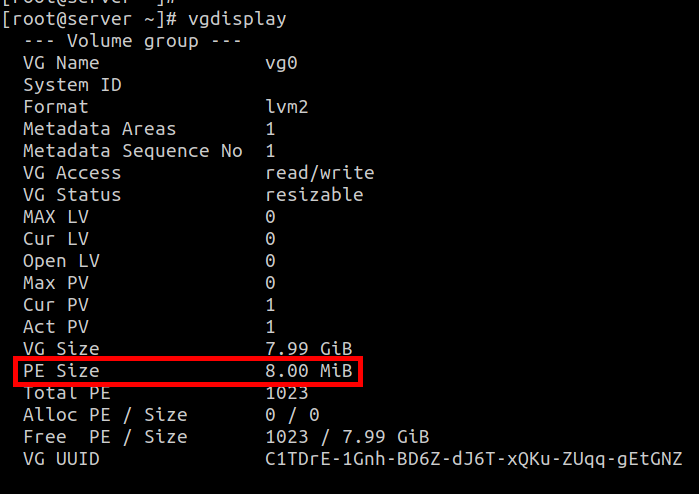
\includegraphics[scale=.4]{content/chapter9/images/pe1.png}
			\caption{PE size changed}
			\label{fig:PE size4}
		\end{figure}
	
		
		\item \textbf{You cannot change PE size once the VG is created}.
		
	\end{itemize}



\end{flushleft}

\newpage


